\documentclass[12pt,a4paper]{article}

\usepackage[margin=2.2cm]{geometry}
\usepackage{fontspec}
\usepackage{xeCJK}
\setmainfont{Times New Roman}
\setCJKmainfont{DFKai-SB}[AutoFakeBold,AutoFakeSlant]
\setCJKmonofont{DFKai-SB}
\usepackage{amsmath,amssymb,bm}
\usepackage{booktabs}
\usepackage{graphicx}
\usepackage{caption}
\usepackage{setspace}
\captionsetup{font=small,labelfont=bf,skip=4pt}
\graphicspath{{figures/}}
\usepackage{hyperref}
\setstretch{1.08}
\raggedbottom

\hypersetup{colorlinks=true,linkcolor=black,urlcolor=blue}

\begin{document}

\section*{The extension problem}

The point of this note is to connect an abstract right-half-plane (RHP) zero to a motion one can see.
Parts of the original Problem~46 stay labeled ``Problem~46(a)'', ``Problem~46(b)'', and ``Problem~46(c)''.
The extension prompt itself was also written as (a), (b), and (c).
Those labels are renamed here to Extension~1, Extension~2, and Extension~3, so they are not confused with Problem~46.

\begin{enumerate}
  \item[\textbf{Extension 1.}]
  \textbf{Physical model and the mathematical link.}
  Find or derive a classical dynamical system that has a single real RHP zero
  (for example an inverted pendulum on a cart, a rear-wheel-steered vehicle, or balancing a ruler on a fingertip).
  Write the simplified linearized equations of motion.
  Derive the transfer function, locate the poles and zeros explicitly,
  and show that the number of real RHP zeros is odd, which is the condition in Problem~46 under which a step response must undershoot.

  \item[\textbf{Extension 2.}]
  \textbf{Three-dimensional VPython simulation.}
  Build a 3D animation of that system in VPython.
  Start from rest, and for \(t>0\) apply a positive step command in the target.
  The animation should show the trajectory and the attitude.
  In the same VPython session, plot the output (for example the cart position) against time, so the curve can be compared with the animation.

  \item[\textbf{Extension 3.}]
  \textbf{Physical intuition.}
  Using both the derivation and the simulation, describe what the system does at the instant the step is applied,
  and how that motion is the ``wrong-direction'' undershoot on the plot.
  Explain, from inertia, moment balance, and the shift of the center of mass, why the system must first move backward before it can travel toward the target.
  State what goes wrong physically if that initial reverse motion is absent.
\end{enumerate}

The system chosen here is an inverted pendulum on a cart.
\begin{quote}
Animation: \texttt{inverted\_pendulum\_undershoot.py}\\
Video: \url{https://youtu.be/Q5fvMPvR5O4}
\end{quote}

The parameters below are those used in the program:
\[
  M=1.0\,\mathrm{kg},\quad
  m=0.25\,\mathrm{kg},\quad
  L=1.5\,\mathrm{m},\quad
  g=9.81\,\mathrm{m/s^2}.
\]

%==============================================================================
\section{Extension 1: model and transfer function}

\subsection{Linearized equations of motion}

The cart moves on a horizontal track. The position \(x\) is positive to the right, and so is the applied force \(F\).
The rod has length \(L\), with the mass concentrated at the end.
The angle \(\theta=0\) is upright. A positive \(\theta\) puts the bob to the right of the pivot, toward \(+x\).

The bob coordinates are
\[
  x_b=x+L\sin\theta,\qquad y_b=L\cos\theta
\]
(\(y\) upward, pivot height taken as zero).
The potential \(mgy_b=mgL\cos\theta\) is largest at \(\theta=0\), so the upright position is unstable.

Kinetic and potential energy give the Lagrangian
\[
  \mathcal{L}
  =\frac12(M+m)\dot x^2
   +mL\dot x\dot\theta\cos\theta
   +\frac12 mL^2\dot\theta^2
   -mgL\cos\theta.
\]
The Euler--Lagrange equations in \(x\) and \(\theta\), before linearization, are
\begin{align}
  (M+m)\ddot x+mL\ddot\theta\cos\theta-mL\dot\theta^2\sin\theta&=F,
  \label{eq:nl-x}\\
  \ddot x\cos\theta+L\ddot\theta-g\sin\theta&=0.
  \label{eq:nl-th}
\end{align}
The program integrates these two equations.

Near \(\theta=0\), \(\sin\theta\approx\theta\), \(\cos\theta\approx 1\), and the \(\dot\theta^2\) term is second order.
The linearized equations of motion are
\begin{align}
  (M+m)\ddot x+mL\ddot\theta&=F,
  \label{eq:lin-x}\\
  \ddot x+L\ddot\theta-g\theta&=0.
  \label{eq:lin-th}
\end{align}
If the cart is locked (\(\ddot x=0\)), the second equation becomes \(\ddot\theta=(g/L)\theta\).
A small lean grows as \(e^{+\sqrt{g/L}\,t}\).
That growth rate is the same number as the RHP zero derived next.

%==============================================================================
\subsection{Open-loop transfer function}

Laplace transformation of \eqref{eq:lin-x} and \eqref{eq:lin-th} gives
\begin{align}
  (M+m)s^2X+mLs^2\Theta&=F,
  \label{eq:s-x}\\
  s^2X+(Ls^2-g)\Theta&=0.
  \label{eq:s-th}
\end{align}
From \eqref{eq:s-th},
\[
  \Theta=\frac{s^2X}{g-Ls^2}.
\]
Substitution into \eqref{eq:s-x} produces
\begin{equation}
  G(s)=\frac{X(s)}{F(s)}
  =\frac{g-Ls^2}{s^2\bigl[(M+m)g-MLs^2\bigr]}
  =\frac{s^2-g/L}{Ms^2\bigl(s^2-(M+m)g/(ML)\bigr)}.
  \label{eq:G}
\end{equation}
The numerator factors as \(s^2-g/L=(s-\sqrt{g/L})(s+\sqrt{g/L})\).
The zeros are
\begin{equation}
  s=\pm\sqrt{\frac{g}{L}}=\pm\sqrt{6.54}\approx\pm 2.557.
  \label{eq:zeros}
\end{equation}
Only \(+\sqrt{g/L}\) lies in the right half-plane, and it is real.
There is no complex-conjugate pair of zeros.
The open-loop plant therefore has exactly one real RHP zero, an odd number.

The poles come from the denominator:
\begin{equation}
  s=0\ \text{(double)},\qquad
  s=\pm\sqrt{\frac{(M+m)g}{ML}}
   =\pm\sqrt{8.175}\approx\pm 2.859.
  \label{eq:ol-poles}
\end{equation}
One of them, \(+\sqrt{(M+m)g/(ML)}\), is in the right half-plane, and there is also a double pole at the origin.
The open loop is unstable.

Two facts should be kept apart.
The zero \(\sqrt{g/L}\) does not depend on the cart mass or the bob mass. It is fixed by the rod length and gravity, and it is the exponent with which the angle diverges when the cart is held fixed.
The poles do move with \(M\) and \(m\).
The open loop is already strictly proper (the denominator exceeds the numerator by two), but Problem~46(c) also requires stability.
Here one pole is in the right half-plane, and the poles at the origin mean there is no finite dc gain, so \(G(s)\) alone does not imply that a step must undershoot.
That check is made on the closed loop below, where Problem~46(c) applies.

\subsection{Closed loop: the zeros stay, the poles move}

Take the state \((x,\dot x,\theta,\dot\theta)\).
The simulation uses linear state feedback and a position command \(r\),
\begin{equation}
  F=-k_x(x-r)-k_v\dot x-k_\theta\theta-k_\omega\dot\theta,
  \label{eq:u}
\end{equation}
with the closed-loop poles placed at
\[
  -3.5,\ -4,\ -4.8,\ -5.6.
\]
The characteristic polynomial is
\begin{align}
  \chi(s)&=(s+3.5)(s+4)(s+4.8)(s+5.6) \nonumber\\
         &=s^4+17.9s^3+118.88s^2+347.2s+376.32.
  \label{eq:chi}
\end{align}
All four roots have negative real parts, so the closed loop is stable.

State feedback does not move the transmission zeros from \(F\) to \(x\), and it does not change the high-frequency coefficient of relative degree \(2\).
The open loop satisfies \(s^2G(s)\to 1/M=1\), and the same leading coefficient remains after feedback:
\[
  \frac{X(s)}{F(s)}=\frac{s^2-g/L}{\chi(s)}.
\]
The command enters through the term \(+k_x r\) in \eqref{eq:u}.
Call that coefficient \(N\) (in the program, \(N=k_x\)). Then
\begin{equation}
  T(s)=\frac{X(s)}{R(s)}=N\,\frac{s^2-g/L}{\chi(s)}.
  \label{eq:T}
\end{equation}
The zeros of \(T(s)\) are still \(\pm\sqrt{g/L}\).
Unit dc gain, so that the cart stops at the commanded position, requires
\[
  T(0)=N\frac{-g/L}{\chi(0)}=1.
\]
A stable monic polynomial factors into terms \((s+a)\) and \(s^2+bs+c\) with positive coefficients, so \(\chi(0)>0\). Hence
\begin{equation}
  N=-\chi(0)\,\frac{L}{g}
   =-376.32\times\frac{1.5}{9.81}
   =-57.541<0.
  \label{eq:N}
\end{equation}
The position gain is negative because this normalization requires it.
Substituting the value of \(N\),
\begin{equation}
  T(s)=\frac{-57.541\,s^2+376.32}{s^4+17.9s^3+118.88s^2+347.2s+376.32}
      =-57.541\,\frac{(s-2.557)(s+2.557)}{\chi(s)}.
  \label{eq:Tnum}
\end{equation}
The only real zero in the right half-plane is \(s=+2.557\).
The zero \(-2.557\) is in the left half-plane.
The denominator has degree \(4\) and the numerator degree \(2\), so \(T(s)\) is strictly proper.

Those are the three hypotheses of Problem~46(c): stable, strictly proper, and an odd number of real RHP zeros.
The steady state of a unit step is \(T(0)=1>0\), but the response must start in the negative direction.

The initial direction matches the definition in Problem~46(c), rather than the sketches of \(G_1\) and \(G_2\) asked for in Problem~46(a).
The relative degree is \(2\), so \(x(0)=\dot x(0)=0\), and the first nonzero derivative is
\[
  \ddot x(0^+)=\lim_{s\to\infty}s^2T(s)=N=-57.541<0.
\]
The steady state is \(+1\,\mathrm{m}\), while the initial acceleration is negative: the response starts the wrong way.
The sign uses only \(\chi(0)>0\) and the zeros \(\pm\sqrt{g/L}\). It does not depend on the particular locations of these four poles.
Any stable closed loop with positive dc gain starts the step by moving toward \(-x\).

%==============================================================================
\section{Extension 2: simulated trajectories}

This section records the trajectories from the animation, for comparison in Extension~3.
It is not Problem~46(b). Problem~46(b) asks why the transients of \(G_1\) and \(G_2\) differ.

The program starts at rest, \((x,\dot x,\theta,\dot\theta)=(0,0,0,0)\), holds that state until \(t=0\), and then switches the command to \(r=+1\,\mathrm{m}\).
The integrator uses the nonlinear equations \eqref{eq:nl-x} and \eqref{eq:nl-th}. Only the controller is the linear gain above.
On screen the cart, the rod angle, and the ground tracks all move, while \(x(t)\) is drawn on the same time axis. A second plot shows \(\theta(t)\).
The three-dimensional run is recorded at \url{https://youtu.be/Q5fvMPvR5O4}:
as soon as the step is applied, the force arrow points toward \(-x\), the cart and its cyan track move left, and the bob leans toward the target.

A few samples of the nonlinear trajectory:

\begin{center}
\begin{tabular}{@{}cccc@{}}
\toprule
\(t\) (s) & \(x\) (m) & \(\theta\) (deg) & \(F\) (N) \\
\midrule
\(0^+\)   & \(0\)      & \(0\)        & \(-57.5\) \\
\(0.05\)  & \(-0.053\) & \(+2.0\)     & \(-18.1\) \\
\(0.20\)  & \(-0.318\) & \(+12.7\)    & \(+17.6\) \\
\(0.25\)  & \(-0.343\) & \(+14.1\)    & \(+17.8\) \\
\(0.50\)  & \(+0.024\) & \(+6.7\)     & \(+1.2\) \\
\(1.0\)   & \(+0.829\) & \(-6.5\)     & \(-3.0\) \\
\(4.0\)   & \(+1.000\) & \(\approx 0\) & \(\approx 0\) \\
\bottomrule
\end{tabular}
\end{center}

\begin{figure}[ht]
  \centering
  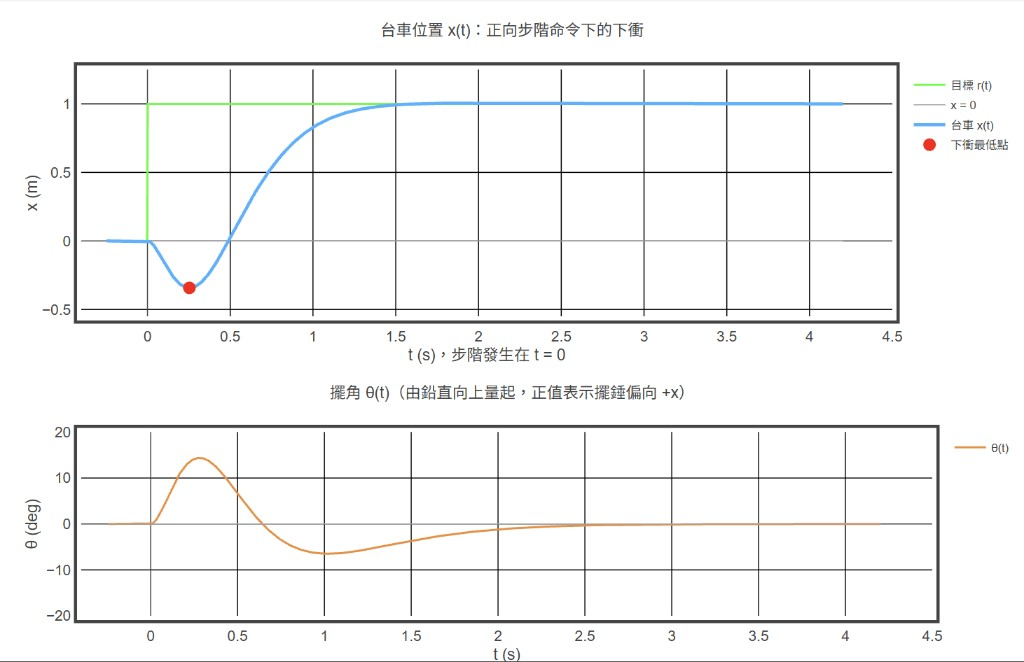
\includegraphics[width=0.92\textwidth]{sim_xt_theta.png}
  \caption{Cart position and lean angle drawn by VPython on the same run.
  After the command jumps to \(+1\,\mathrm{m}\) at \(t=0\), \(x\) first falls to about \(-0.34\,\mathrm{m}\) (red marker) while \(\theta\) rises to about \(+14^\circ\). The cart then returns to the target.}
  \label{fig:sim}
\end{figure}

\begin{figure}[ht]
  \centering
  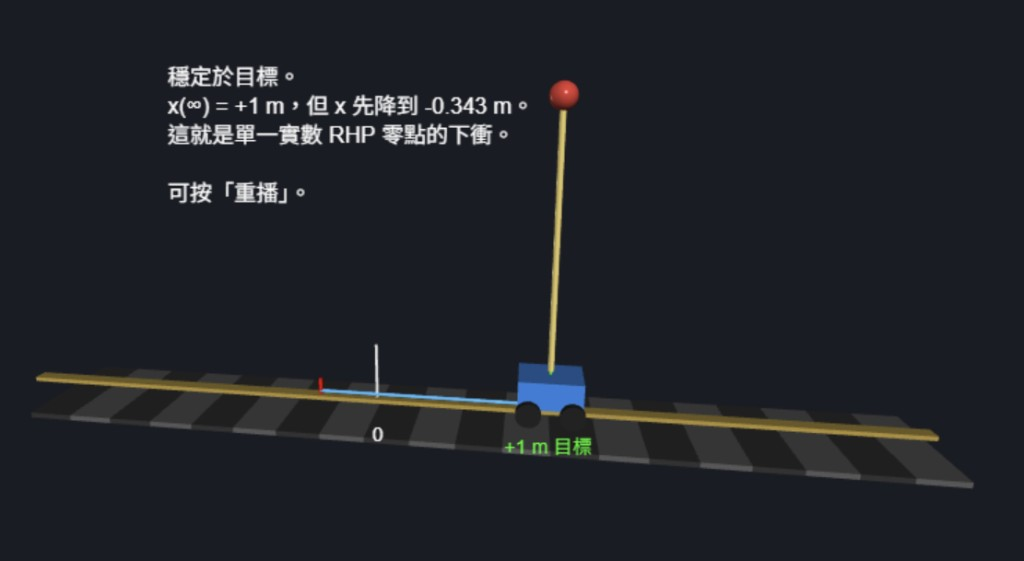
\includegraphics[width=0.88\textwidth]{sim_cart.png}
  \caption{The 3D scene after the step has settled. The cart is at \(+1\,\mathrm{m}\) and the pendulum is upright again. The cyan curve is the cart track; the red marker on the left is the undershoot minimum, \(x=-0.343\,\mathrm{m}\).}
  \label{fig:cart}
\end{figure}

Figure~\ref{fig:sim}, Fig.~\ref{fig:cart}, and the table are the same nonlinear trajectory.
The position \(x\) reaches about \(-0.34\,\mathrm{m}\) near \(t=0.25\,\mathrm{s}\), then crosses the origin and settles at \(+1\,\mathrm{m}\).
The positive peak of \(\theta\), about \(+14^\circ\), occurs while the cart is still on the far side of the target.
Near \(t=1\,\mathrm{s}\) the angle is about \(-6.5^\circ\): the cart has started chasing to the right and is pulling the pendulum back.
Throughout the run \(|\theta|\) stays within about \(14.4^\circ\), so the linear design and the nonlinear motion on the screen stay in the same regime.
The curve \(x(t)\) crossing below zero is the undershoot defined in Problem~46(c). It is the same event as the cart moving left in the video.

%==============================================================================
\section{Extension 3: why the first motion must be backward}

Extension~3 reads the trajectories of Extension~2 mechanically.
It does not reprove the if-and-only-if statement of Problem~46(c).
It uses the initial direction that theorem already guarantees, and explains why the cart has to move toward \(-x\).

\subsection{What happens at the step}

Before \(t=0\) the system is at rest and the pendulum is upright.
When the command switches to \(+1\,\mathrm{m}\), the force is immediately \(-57.5\,\mathrm{N}\) and the arrow points left.
The cart slides toward \(-x\), and the cyan ground track grows to the left.
Over that same interval, \(x(t)\) in Fig.~\ref{fig:sim} falls from zero to a minimum near \(-0.34\,\mathrm{m}\).
The curve going down is the cart itself moving away from the target.

The rod leans toward the target at the same time.
By definition, \(\theta>0\) means the bob is to the right of the pivot.
At \(t=0.2\,\mathrm{s}\) the cart is already at \(-0.32\,\mathrm{m}\), but \(\theta\) is about \(+13^\circ\): the pivot is on the left and the bob is to its right, leaning toward \(+1\,\mathrm{m}\).
Once that lean exists, the force reverses and the cart turns around to chase the bob.
Only then does \(x(t)\) climb out of the trough, and both \(x\) and \(\theta\) settle at \((x,\theta)=(1,0)\).

\subsection{Inertia and moment balance}

No external force pushes the bob directly.
The only horizontal external force acts on the cart. The bob is moved through the rod.

At the instant the command is applied, \(\theta=\dot\theta=0\). Rewrite \eqref{eq:lin-th} as
\begin{equation}
  \ddot\theta=\frac{g}{L}\theta-\frac{1}{L}\ddot x,
  \label{eq:thdd}
\end{equation}
so that \(\ddot\theta(0^+)=-\ddot x(0^+)/L\).
A positive \(\theta\), a lean toward the target, requires \(\ddot\theta(0^+)>0\), hence \(\ddot x(0^+)<0\).
The pivot must accelerate to the left.
The horizontal velocity of the bob cannot jump, so when the pivot runs left the bob is left behind on the right side of the pivot.
That is the simultaneous rise of \(\theta\) and drop of \(x\) in the video.

After \(\theta>0\), the gravity term \((g/L)\theta\) has the same sign as \(\theta\).
The upright position is the top of the potential, so gravity does not restore the pendulum. It increases the lean to the right.
The cart is then accelerated toward \(+x\). The pivot catches up with the bob, \(\ddot x>0\) contributes a negative angular acceleration in \eqref{eq:thdd}, \(\theta\) is brought back to zero, and the net displacement of the system is toward the target.
In the table, the force has already become positive by \(t=0.2\,\mathrm{s}\) while \(x\) is still negative. That is the interval in which the lean is large enough and the chase has started.

The center of mass also moves left at first.
The horizontal external force sets the acceleration of the system center of mass, so \(F(0^+)<0\) means the center of mass initially accelerates toward \(-x\).
Relative to the cart, the center of mass is shifted toward the bob:
\[
  x_{\mathrm{cm}}=x+\frac{mL}{M+m}\sin\theta.
\]
While \(\theta>0\) the bob is to the right of the cart, so the cart is farther left than the center of mass and the undershoot in \(x\) is deeper than the undershoot of the center of mass.
The final state \(\theta=0\), \(x=+1\) also places the center of mass at \(+1\,\mathrm{m}\).
The later positive force supplies the impulse that reverses the initial leftward momentum.
The first force still has to be negative. Otherwise the lean has the wrong sign.

\subsection{If the reverse motion is missing}

If the step is met with \(\ddot x(0^+)\ge 0\), then \(\ddot\theta(0^+)\le 0\) and \(\theta\) immediately becomes negative.
The bob falls to the left of the pivot, away from the target.
The gravity term \((g/L)\theta\) is then negative and increases \(|\theta|\). The pendulum falls on the wrong side.

The equilibrium that was asked for is \(x=+1\) together with \(\theta=0\) and zero angular rate.
If the cart stops while \(\theta\) is still negative, the gravity term in \eqref{eq:thdd} keeps pulling the pendulum down, so the upright position is not an equilibrium of that state.
Recovering a negative \(\theta\) still requires an interval with \(\ddot x<0\): the cart must accelerate backward anyway, only later, and after the lean has already grown.
The linear model is useful only within about fifteen degrees. Once the pendulum has clearly fallen the wrong way, that equilibrium has been left.

The reverse motion is therefore not an accident of this particular gain.
The conditions \(T(0)>0\) and \(\ddot x(0^+)=N<0\) are fixed by the zero \(\sqrt{g/L}\):
every loop that keeps the poles in the left half-plane and the dc gain positive starts the step toward \(-x\).
Without that first move, the lean has the opposite sign from the target, gravity carries the pendulum away from upright, and the state ``cart at \(+1\,\mathrm{m}\), pendulum upright'' is not reached.

\end{document}
